\section{Results}\label{sec:results}

This section presents the experimental results and their implications for short-term prediction of Brazilian Mini-Index futures. Following the organization of the precursor, it first describes the common experimental setup and then discusses the performance of the individual model families. The expanded benchmark subsequently reports the direct cross-model comparison, exploratory statistical evidence, and economic outcomes.

\subsection{Experimental Setup and Data Partitioning}

All model--optimizer combinations use the seven descriptors described in Section~\ref{sec:featureselection}, the chronological split shown in Figure~\ref{fig:partition}, and the same 1,000-evaluation allowance per seed. RF, SVM, MLP, and 1D-CNN each are searched with RS, GA, PSO, DE, and GWO. The two protocols differ only in the validation fitness used to rank candidate configurations. Three common seeds (1--3) are available for every cell in both protocols.

Consequently, the direct comparison between fitness functions is descriptive: each reported model--optimizer result is the mean over the same three seeds. The locked test block contains 3,012 observations and is not used during search. This design differs from the randomized training and test sampling used in the precursor and removes look-ahead exposure from model selection.

\subsection{Performance of the Models}
\label{sec:performance_models}

Tables~\ref{tab:rf_hyperparameters}--\ref{tab:cnn_hyperparameters} retain the presentation pattern of the precursor: each table states the search space and an illustrative GA-selected configuration. The configurations are from seed 1 under Protocol A and are included to make the optimization procedure concrete; they are not asserted to be universally optimal because all optimizer--seed outcomes are summarized below.

\begin{table}[htbp]
\centering
\caption{Random Forest hyperparameters and representative GA-selected configuration.}
\label{tab:rf_hyperparameters}
\small
\begin{tabular}{lcc}\toprule
\textbf{Hyperparameter} & \textbf{Search space} & \textbf{Selected value}\\\midrule
$n_{\mathrm{estimators}}$ & $[50,500]$ & 58\\
$\mathrm{max\_depth}$ & $[5,50]$ & 6\\
$\mathrm{min\_samples\_split}$ & $[2,20]$ & 13\\
$\mathrm{min\_samples\_leaf}$ & $[1,20]$ & 15\\
$\mathrm{max\_features}$ & $\{\mathrm{sqrt},\mathrm{log2},\mathrm{None}\}$ & None\\
$\mathrm{class\_weight}$ & $\{\mathrm{None},\mathrm{balanced}\}$ & None\\\bottomrule
\end{tabular}
\end{table}

\begin{table}[htbp]
\centering
\caption{SVM hyperparameters and representative GA-selected configuration.}
\label{tab:svm_hyperparameters}
\small
\begin{tabular}{lcc}\toprule
\textbf{Hyperparameter} & \textbf{Search space} & \textbf{Selected value}\\\midrule
$C$ & $[10^{-3},10^{3}]$ (log scale) & 2.089\\
$\gamma$ & $[10^{-5},10^{1}]$ (log scale) & 5.044\\
Kernel & $\{\mathrm{linear},\mathrm{RBF}\}$ & linear\\\bottomrule
\end{tabular}
\end{table}

\begin{table}[htbp]
\centering
\caption{MLP hyperparameters and representative GA-selected configuration.}
\label{tab:mlp_hyperparameters}
\small
\begin{tabular}{lcc}\toprule
\textbf{Hyperparameter} & \textbf{Search space} & \textbf{Selected value}\\\midrule
Hidden neurons & $[5,500]$ & 410\\
Learning rate & $[10^{-8},10^{-2}]$ (log scale) & $3.42\times10^{-4}$\\
$L_2$ regularization & $[10^{-8},10^{-2}]$ (log scale) & $1.66\times10^{-7}$\\
Dropout rate & $[0,0.10]$ & 0.057\\
Batch size & $\{16,32,64,80,112,128\}$ & 112\\\bottomrule
\end{tabular}
\end{table}

\begin{table}[htbp]
\centering
\caption{1D-CNN hyperparameters and representative GA-selected configuration.}
\label{tab:cnn_hyperparameters}
\small
\begin{tabular}{lcc}\toprule
\textbf{Hyperparameter} & \textbf{Search space} & \textbf{Selected value}\\\midrule
Filters & $[8,128]$ & 48\\
Kernel size & $[2,5]$ & 3\\
Dense neurons & $[16,256]$ & 251\\
Learning rate & $[10^{-8},10^{-2}]$ (log scale) & $3.90\times10^{-6}$\\
$L_2$ regularization & $[10^{-8},10^{-2}]$ (log scale) & $5.70\times10^{-6}$\\
Dropout rate & $[0,0.10]$ & 0.026\\
Batch size & $\{16,32,64,80,112,128\}$ & 16\\\bottomrule
\end{tabular}
\end{table}

Figures~\ref{fig:rf_convergence}--\ref{fig:cnn_convergence} replace the three GA-only convergence plots of the precursor with the five budget-matched search trajectories. For each model, the left panel follows the compound MCC/$F_1$ fitness and the right panel follows weighted training/validation accuracy. The vertical scales differ because the objectives differ; their role is to show search convergence within a protocol, not to compare objective magnitudes across protocols.

\begin{figure}[htbp]\centering
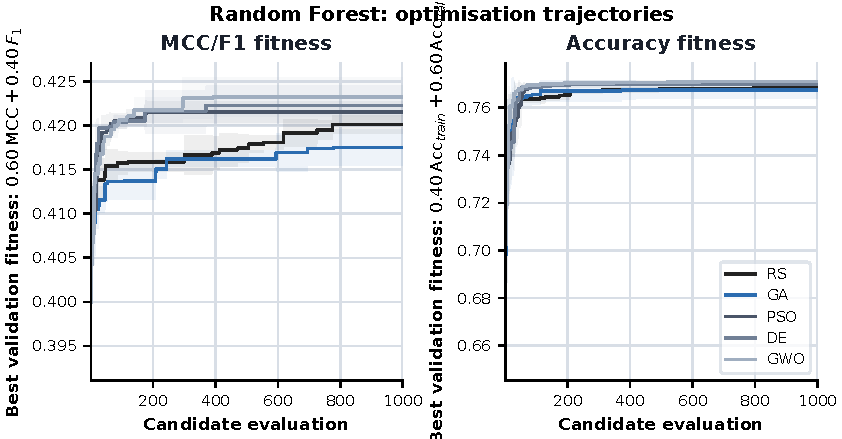
\includegraphics[width=0.93\linewidth]{figures/ijcnn_style_rf_convergence.pdf}
\caption{Fitness evolution during equal-budget optimization of the Random Forest model. Lines summarize the three common seeds.}
\label{fig:rf_convergence}\end{figure}

\begin{figure}[htbp]\centering
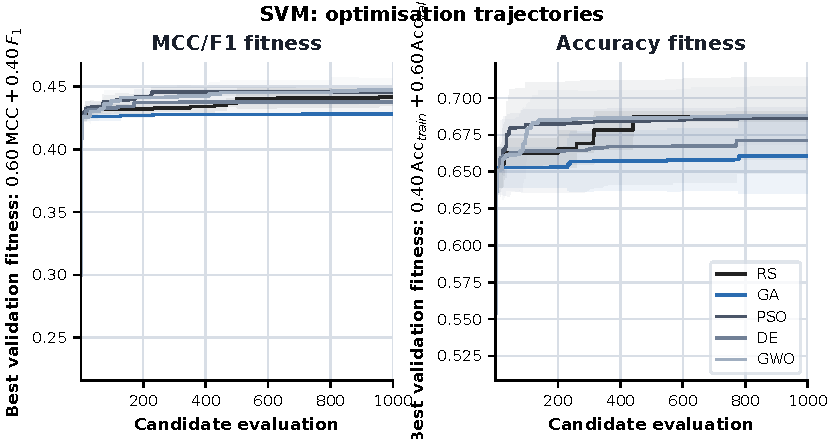
\includegraphics[width=0.93\linewidth]{figures/ijcnn_style_svm_convergence.pdf}
\caption{Fitness evolution during equal-budget optimization of the SVM model. Lines summarize the three common seeds.}
\label{fig:svm_convergence}\end{figure}

\begin{figure}[htbp]\centering
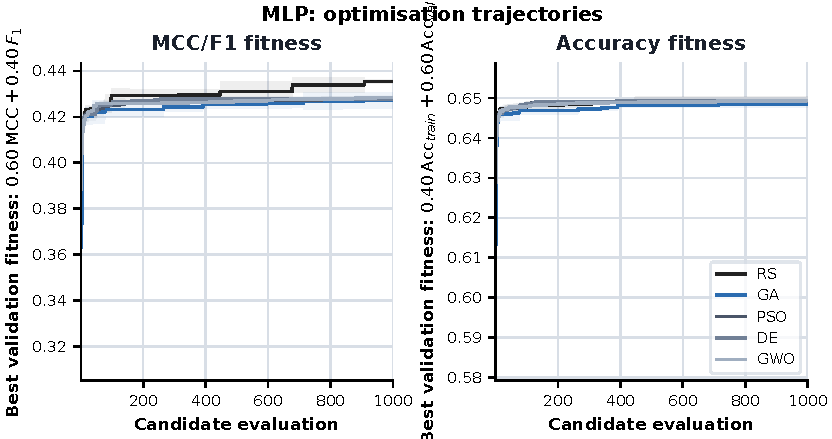
\includegraphics[width=0.93\linewidth]{figures/ijcnn_style_mlp_convergence.pdf}
\caption{Fitness evolution during equal-budget optimization of the MLP model. Lines summarize the three common seeds.}
\label{fig:mlp_convergence}\end{figure}

\begin{figure}[htbp]\centering
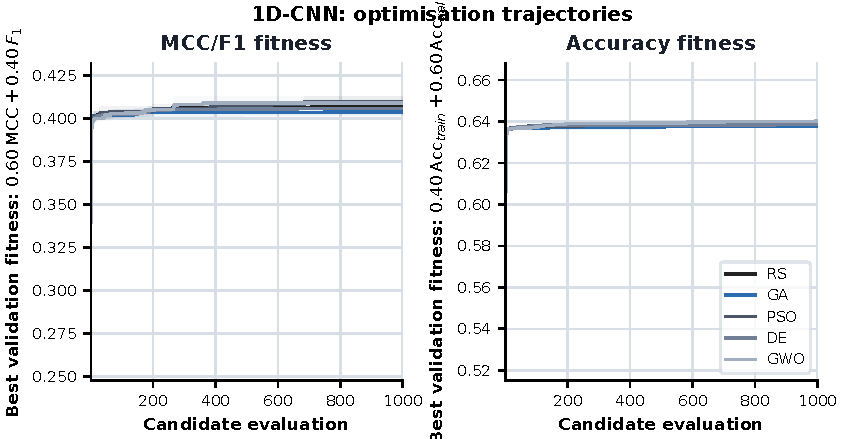
\includegraphics[width=0.93\linewidth]{figures/ijcnn_style_cnn_convergence.pdf}
\caption{Fitness evolution during equal-budget optimization of the 1D-CNN model. Lines summarize the three common seeds.}
\label{fig:cnn_convergence}\end{figure}

Table~\ref{tab:predictive_summary} and Figure~\ref{fig:model_comparison} present held-out performance aggregated over 15 optimizer--seed blocks per model within each protocol. Under MCC/$F_1$ fitness, RF has the largest mean test accuracy (0.645), MCC (0.289), and $F_1$ (0.664). Under weighted accuracy fitness, MLP has the largest mean test accuracy (0.651), MCC (0.301), and $F_1$ (0.658). The reversal reinforces that the validation criterion and model family should be reported separately rather than treated as interchangeable.

\begin{table}[htbp]
\centering
\caption{Mean locked-test predictive outcomes by backbone and validation protocol (15 optimizer--seed blocks per row).}
\label{tab:predictive_summary}
\small
\begin{tabular}{lccc|ccc}\toprule
& \multicolumn{3}{c|}{\textbf{MCC/$F_1$ fitness}} & \multicolumn{3}{c}{\textbf{Weighted accuracy fitness}}\\
\textbf{Model} & Accuracy & MCC & $F_1$ & Accuracy & MCC & $F_1$\\\midrule
RF & 0.645 & 0.289 & 0.664 & 0.604 & 0.208 & 0.624\\
SVM & 0.604 & 0.214 & 0.602 & 0.578 & 0.159 & 0.600\\
MLP & 0.630 & 0.261 & 0.639 & 0.651 & 0.301 & 0.658\\
1D-CNN & 0.613 & 0.224 & 0.597 & 0.635 & 0.271 & 0.639\\\bottomrule
\end{tabular}
\end{table}

\begin{figure}[htbp]\centering
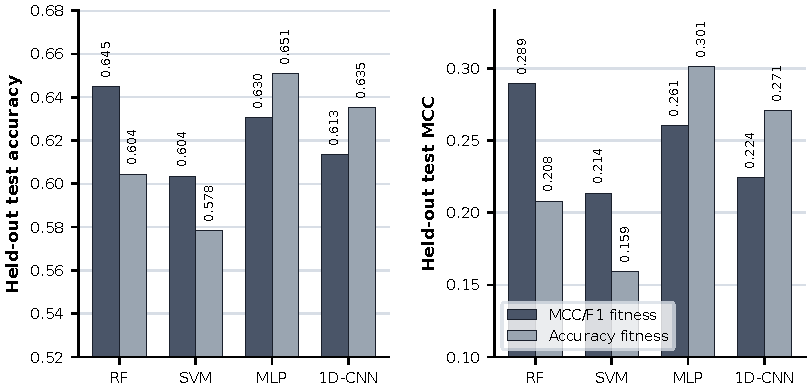
\includegraphics[width=0.94\linewidth]{figures/ijcnn_style_model_performance.pdf}
\caption{Comparison of mean locked-test accuracy and MCC for all four model families under the two validation objectives.}
\label{fig:model_comparison}\end{figure}

\subsection{Exploratory Statistical and Economic Evaluation}

The model-level tests are performed within each holdout protocol. The five optimizer--seed combinations yield 15 matched blocks for each backbone. Under MCC/$F_1$ fitness, the Friedman comparison of test MCC is significant ($\chi^2=22.84$, $p=4.36\times10^{-5}$), with RF obtaining the best mean outcome. Under weighted accuracy fitness, the comparison of test accuracy is significant ($\chi^2=42.92$, $p=2.56\times10^{-9}$), with MLP first; its Holm-adjusted pairwise contrasts against RF, SVM, and 1D-CNN are significant ($p_{\mathrm{Holm}}\approx0.00194$). These tests compare models within a protocol and should not be interpreted as a confirmatory test between the two fitness functions.

The economic evaluation yields a complementary ranking. Under MCC/$F_1$ fitness, RF has the largest mean total profit (26,465 points). Under weighted accuracy fitness, MLP has the largest mean total profit (27,737 points), whereas RF has the least negative mean maximum drawdown (-1,866 points). Figure~\ref{fig:economic_comparison} therefore makes explicit the difference between predictive ranking and return-risk ranking.

\begin{figure}[htbp]\centering
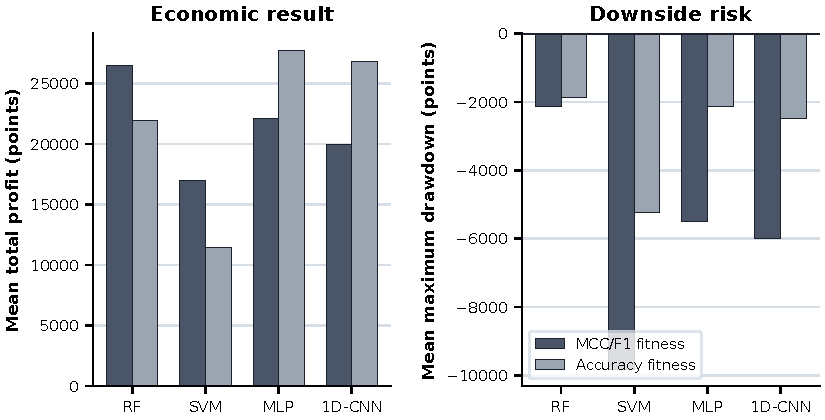
\includegraphics[width=0.94\linewidth]{figures/ijcnn_style_economic_summary.pdf}
\caption{Mean total profit and maximum drawdown across 15 optimizer--seed blocks per model. Results are reported separately for the two validation objectives.}
\label{fig:economic_comparison}\end{figure}
